
\documentclass{article}
\setcounter{secnumdepth}{0}
\usepackage[T1]{fontenc}
\usepackage[utf8]{inputenc}

\usepackage{float}
\usepackage[english]{babel}
\usepackage{tcolorbox}
\usepackage{url}
\usepackage{etoolbox}
\usepackage{multicol}
\usepackage{graphicx}
\usepackage{tabularx}
\usepackage{geometry}
\graphicspath{ {./img/} }

\usepackage{listings}
\usepackage{color}
\definecolor{dkgreen}{rgb}{0,0.6,0}
\definecolor{gray}{rgb}{0.5,0.5,0.5}
\definecolor{mauve}{rgb}{0.58,0,0.82}


\setlength{\parindent}{0em}
\setlength{\parskip}{1em}


\title{Beskrivelse av Real-Time prosjekt \large\\
DSA3102-1 20H Intelligente sanntidssystemer}
\date{\today}

\begin{document}
\selectlanguage{english}
\maketitle
\thispagestyle{empty}
%\centering
\begin{center}

\includegraphics[width=\linewidth,height=0.2\textheight,keepaspectratio]{USN.png}
\end{center}


\newpage
\section{Group members}
	\begin{itemize}
		\item{Stian Onarheim}
		\item{Kent Odde}
		\item{Tarald Vestbøstad}
	\end{itemize}
%\newpage
\section{Description}
	Autonomous vehicle with attached antibac for driving on tables or floor.\\
	Proximity sensors forward/backward and sloped forward/backward.\\
	It has servos to automatically dispense a small amount of antibac if a hand is detected. It has a pressure plate to detect if the antibac is empty. When the antibac container is running low, the car will trigger an alarm. 

	Initially the car will drive in a random direction until it either meets a wall or a cliff, which will result in a change in direction. It will over time build a map of the area, and therafter visit each possible location in sequence, perhaps by making use of a graph theory algorithm like Dijkstra.

\subsection{Prototype drawing}

\begin{figure}[H]
	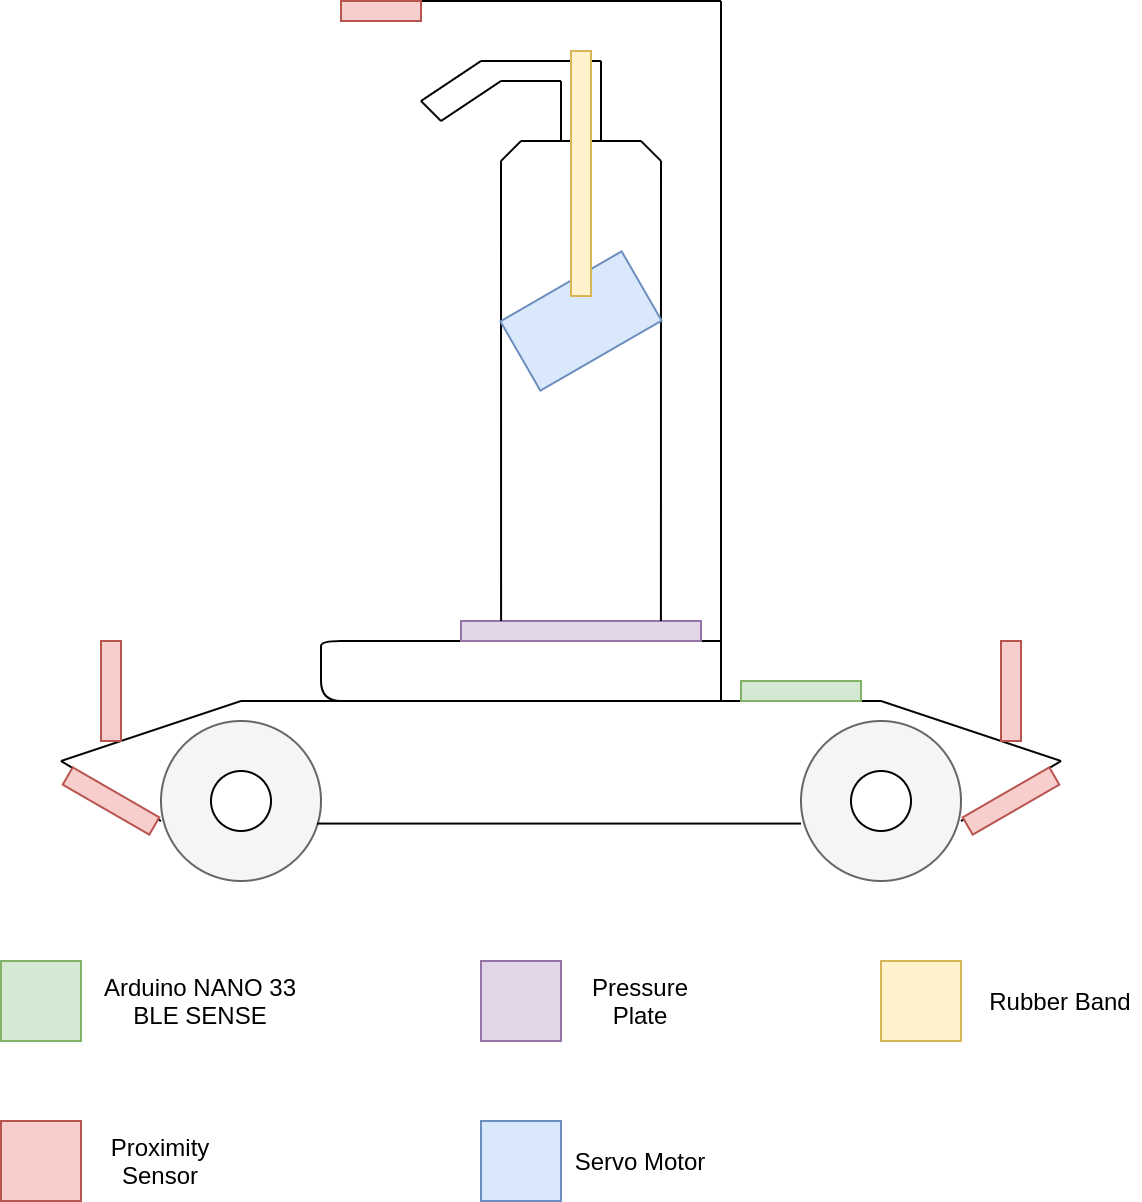
\includegraphics[width=\linewidth]{prototype-drawing.png}
\end{figure}
\newpage

\section{Hardware}
	\begin{itemize}
		\item{Four wheels}
		\item{Chassis}
		\item{Wheel steering}
		\item{Rear wheel drive}
		\item{Weight sensor / pressure plate}
		\item{Four or five extra proximity sensors}
		\item{Two servos for squeezing antibac}
	\end{itemize}
%\newpage
\section{Budget}
\begin{table}[H]
\begin{tabular}{lll}
\textbf{Vare} & \textbf{Pris} & \textbf{URL}      \\
Antibac       & 119,9         & https://bit.ly/3hdS8GH \\
              &               &                   \\
              &               &                  
\end{tabular}
\end{table}
\end{document}




